\documentclass{beamer}

%\usetheme{default}
\usetheme{Frankfurt}
\usecolortheme{default}%{seagull}
\usefonttheme[onlylarge]{structurebold}
\setbeamerfont*{frametitle}{size=\normalsize,series=\bfseries}
\setbeamertemplate{navigation symbols}{}

\usepackage[spanish]{babel}
\usepackage[latin1]{inputenc}
\usepackage{times}
\usepackage[T1]{fontenc}
\usepackage{multicol}
\usepackage{tikz}
\usepackage{graphics}
\usepackage{multirow}
\usetikzlibrary{arrows}
\usepackage{multimedia}
\tikzstyle{block}=[draw opacity=0.7,line width=1.4cm]

\newcommand{\redalert}[1]
{
	{\color[rgb]{1,0,0}{#1}}
}

\newcommand{\Titulo}[1]
{
	\begin{center}
		\tikz \draw (0,0) node[fill=green!50,draw]
		{#1};
	\end{center}
}

\title{Graphs with few trivial critical ideals}
\author{Carlos A. Alfaro}
\date{}


\begin{document}

\begin{frame}

	\maketitle

	\vspace{-2cm}

	\begin{center} 
		
\includegraphics[height=1.5cm]{logo-banxico.jpg}
	\end{center}	
\end{frame}


\begin{frame}
	\tableofcontents
\end{frame}


\section{Assumptions}
\subsection*{S}

\begin{frame}
	\begin{columns}[c]
		\column{.5\textwidth}
			\begin{block}{Assumptions on graphs}
				\begin{itemize}
					\item<1> are \alert{connected},
					\item<2> \alert{multiple edges} are allowed, and
					\item<3> \alert{loops} are forbidden. 
					%\item<3> Sumidero
				\end{itemize}
			\end{block}
		\column{.3\textwidth}
			\begin{tabular}{c}
				\visible<1>{
					\begin{tikzpicture}[scale=1]
						\draw (-30:1) node[fill=black!20, draw=black, minimum size=2mm, circle, line width = .3mm] (v1) {\tiny $G_1$};
	    					\draw (90:1)  node[fill=black!20, draw=black, minimum size=2mm, circle, line width = .3mm] (v2) {\tiny $G_2$};
	    					\draw (210:1) node[fill=black!20, draw=black, minimum size=2mm, circle, line width = .3mm] (v3) {\tiny $G_3$};
	    					\draw (-1,1) node (no) {};
	    					\draw (-1,-1) node (so) {};
	    					\draw (1,1) node (ne) {};
	    					\draw (1,-1) node (se) {};
	    					\draw (no) edge[red,line width=.1cm] (se);
	    					\draw (so) edge[red,line width=.1cm] (ne);
		    			\end{tikzpicture}
				} \\
				\visible<2-3>{
					 \begin{tikzpicture}[scale=1]
						\tikzstyle{every node}=[fill=black!20, draw=black, minimum size=2mm, circle, line width = .3mm]
						\path (-30:1) node (v1) {};
	    					\path (90:1)  node (v2) {};
	    					\path (210:1) node (v3) {};
		    				\draw[line width = .3mm] (v1) -- (v2) -- (v3);
		    				\draw (v1) edge[bend left, green, line width = .3mm] (v3);
		    				\draw (v1) edge[bend right,green, line width = .3mm] (v3);
		    				\draw[red, dashed, line width = .3mm] (v2) .. controls (2,1.5) and (2,0.5) .. (v2);
		    	\end{tikzpicture} 
	    			} \\
			\end{tabular}
	\end{columns}
\end{frame}


\section{Motivation: Critical group}


\subsection*{Laplacian matrix}


\begin{frame}
	
	\frametitle{Laplacian Matrix}
	
	\begin{Definition}
		Let $G=(V,E)$ be a graph, the \alert{Laplacian matrix} $L(G)$ of $G$ is the matrix with rows and columns indexed by the vertices of $G$ given by
	\[
	L(G)_{u v}=
	\begin{cases}
	\deg_G(u) & \text{ if } u=v,\\
	-m_{u v} & \text{ otherwise},
	\end{cases}
	\]
	where \alert{$\deg_G(u)$} denote the degree of $u$, and \alert{$m_{u v}$} denote the number of edges from $u$ to $v$.
	\end{Definition}
	
	\begin{columns}[c]
		\column{.3\textwidth}
			\begin{tikzpicture}[scale=.8]
				\tikzstyle{every node}=[inner sep=0pt, minimum width=5pt,draw, circle, fill=black] 
 				\draw (1,-1) node[label=left:{\small $v_1$}] (v1) {};
 				\draw (1,1) node[label=below left:{\small $v_2$}] (v2) {}; 	
 				\draw (3,1) node[label=right:{\small $v_3$}] (v3) {};
 				\draw (3,-1) node[label=right:{\small $v_5$}] (v4) {};
 				\draw (4,0) node[label=right:{\small $v_4$}] (v5) {};
 				\draw (2,-1) node[label=left:{\small $v_6$}] (s) {};
 				\draw (v1) -- (v2) -- (v3) -- (v5) -- (v4)
 				(v2) -- (s) -- (v3);
			\end{tikzpicture}
			
		\column{.7\textwidth}
			$\tiny
			L(G,X_G) = \left[
			\begin{array}{cccccc}
				1 & -1 & 0 & 0 & 0 & 0\\
				-1 & 3 & -1 & 0 & 0 & -1 \\
				0 & -1 & 3 & -1 & 0 & -1 \\
				0 & 0 & -1 & 2 & -1 & 0 \\
				0 & 0 & 0 & -1 & 1 & 0 \\
				0 & -1 & -1 & 0 & 0 & 2 \\
			\end{array}
			\right]		
			$
	\end{columns}
	
\end{frame}


\begin{frame}

	\begin{Definition}
		By considering $L(G)$ as a linear operator on $\mathbb Z^n$, the \alert{critical group} $K(G)$ of $G$ is the torsion part of the cokernel of $L(G)$.
		\[
			coker(L(G))= \mathbb{Z}^{n}/{\sf Im}L(G) = \mathbb{Z}\oplus \alert{K(G)}.
		\]
	\end{Definition}

\end{frame}


\subsection{Invariant factors}


\begin{frame}

	\frametitle{Invarian factors}	
	
	\begin{Theorem}
		\[
			K(G) \cong \mathbb{Z}_{\alert{f_1}} \oplus \mathbb{Z}_{\alert{f_2}} \oplus \cdots \oplus\mathbb{Z}_{\alert{f_{n-1}}},
		\]
		where \alert{$f_i \leq 0$} and  \alert{$f_i \mid f_j$} for all \alert{$i\leq j$}.
	\end{Theorem}
	
	\pause
	
	\begin{Definition}
    The \alert{$f_1, f_2, ..., f_{n-1}$} are called \alert{invariant factors}.
	\end{Definition}
	
	\pause
	
	\begin{block}{Proposition}
		If \alert{$\Delta_i(G)$} is the g.c.d of the $i$-minors of $L(G)$, then \alert{$f_i$} is equal to $\Delta_i(G)/ \Delta_{i-1}(G)$, where $\Delta_0(G)=1$.  
	\end{block}
	
\end{frame}

\subsection{The family $\mathcal G_i$}


\begin{frame}
	\frametitle{The family $\mathcal G_i$}
	
	\begin{block}{Definition}
		Let \alert{$f_1(G)$} be the number of invariant factors of $L(G)$ equal to $1$.
	\end{block}
	
	\pause
		
	\begin{block}{Definition}
		Let $\alert{\mathcal G_i}$ be the family of \alert{simple connected} graphs with $\alert{f_1(G)=i}$.
	\end{block}
	
	\pause
	
	\begin{block}{Example}
		The following graph belongs to $\redalert{\mathcal G_2}$.
		\begin{center}
			\begin{tabular}{c@{\extracolsep{2cm}}c}
				\multirow{4}{2cm}{
					\begin{tikzpicture}[scale=.9]
						\tikzstyle{every node}=[circle, inner sep=0pt, minimum width=5pt] 	
						\draw (-1,1) node (v1) [draw, fill] {};
						\draw (-1,0) node (v2) [draw, fill] {};
						\draw (0,.5) node (v3) [draw, fill] {};
						\draw (1,1) node (v4) [draw, fill] {};
						\draw (1,0) node (v5) [draw, fill] {};
						\draw (-1.3,1.3) node () {\tiny $v_1$};
						\draw (-1.3,-.3) node () {\tiny $v_2$};
						\draw (0,0.2) node () {\tiny $s$};
						\draw (1.3,1.3) node () {\tiny $v_3$};
						\draw (1.3,-.3) node () {\tiny $v_4$};
						\draw (v1) -- (v2) -- (v3) -- (v4) -- (v5) -- (v3) -- (v1);
					\end{tikzpicture}
				}
				& \\
				&
				$
				{\small
					L(G,s)\sim
					\left[
					\begin{array}{cccc}
						       1      &        0         &           0        &        0        \\
						       0      &        1         &           0        &        0        \\   
						       0      &        0         &           3        &        0        \\
						       0      &        0         &           0        &        3         \\ 
					\end{array}
					\right]
				}
				$\\
				&\\
			\end{tabular}
		\end{center}
	\end{block} 
	
\end{frame}


\begin{frame}
	\begin{figure}
		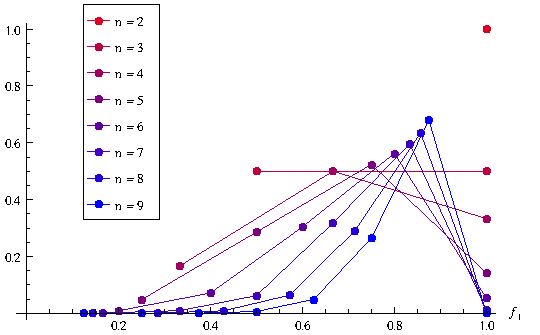
\includegraphics[height=6cm]{InvariantFactors.pdf}
		\caption{\footnotesize Normalized number of graphs with $f_1$ invariant factors equal to 1.}
	\end{figure}
\end{frame}


\begin{frame}
	\begin{block}{Question}
		How often the critical group is cyclic? that is, how often $f_1(G)$ is equal to $n-2$ or $n-1$?
	\end{block}
	
	\pause
	
	\begin{block}{Conjeture (D. Wagner, 2001)}
		Almost every connected simple graph has a cyclic critical group.
	\end{block}
	
	\pause
	
	\begin{Theorem}[M. Wood, 2014]
		The probability that the critical group of a random graph is cyclic is asymptotically at most
		\[
			\zeta(3)^{-1}\zeta(5)^{-1}\zeta(7)^{-1}\zeta(9)^{-1}\zeta(11)^{-1} \cdots \approx 0.7935212
		\]
		where $\zeta$ is the Riemann zeta function.
	\end{Theorem}
\end{frame}


\begin{frame}	
	
	\frametitle{Graphs with one invariant factor equal to 1}
	
	On the other hand...
	
	\pause
	
	\begin{block}{Question}
		\begin{center}
			What we can say about ${\mathcal G_1}$?
		\end{center}
	\end{block}
	
	\pause
	
	\begin{Theorem}[Lorenzini, 1991]
		If $G$ is a \alert{simple connected} graphs, then the following statements are equivalent:
		\begin{enumerate}[i.]
			\item $G \in \mathcal{G}_1$,
			\item $G$ is $P_3$-free, where \alert{$P_n$} denote the path with $n$ vertices,
			\item $G$ is a complete graph.
		\end{enumerate}
	\end{Theorem}
	
\end{frame}


\subsection{Graphs with more than one invariant factor equal to 1}

\begin{frame}

	\frametitle{Graphs with more than one invariant factor equal to 1}
	
	\begin{block}{Question}
		\begin{center}
			What we can say about ${\mathcal G_2}$ and ${\mathcal G_3}$?
		\end{center}
	\end{block}
	
	\pause
	
	\begin{Theorem}
		Let $G$ be a \alert{simple connected} graph.
		Then, $G\in \mathcal{G}_2$ if and only if $G$ is one of the following graphs:
		\begin{enumerate}[i.]
			\item \alert{$K_{n_1,n_2,n_3}$}, where $n_1$, $n_2$ y $n_3$ have the same parity.
			\item \alert{$L_{n_1,n_2,n_3}$}, where $n_1, n_2, n_3 \geq 3$ have the same parity, and other \alert{eleven special cases}.
			\[
				\begin{tikzpicture}[scale=3]
					\draw[draw=black!40, line width=15pt] (-.5,0) -- (0,0);
					\draw[draw=black!40, line width=15pt] (.5,0) -- (0,0);
					\draw (-.5,0) node[draw, circle, fill=black!40] () {\tiny $K_{n_1}$};
					\draw (0,0) node[draw, circle, fill=white] () {\tiny $T_{n_2}$};
					\draw (.5,0) node[draw, circle, fill=black!40] () {\tiny $K_{n_3}$};
				\end{tikzpicture}
			\]
		\end{enumerate}
	\end{Theorem}
	
	The proof uses critical ideals
\end{frame}


\section{Critical ideals}

\subsection{Definition}

\begin{frame}
	\frametitle{The critical ideals of a graph}
	\begin{Definition}
		Given a graph $G=(V,E)$ and a set of indeterminates $X_G=\{x_u \, : \, u\in V\}$, the \alert{generalised Laplacian matrix} $L(G,X_G)$ of $G$ is the matrix given by
		\[
			L(G,X_G)_{u v}=
			\begin{cases}
				x_u & \text{ if } u=v,\\
				-m_{u v} & \text{ otherwise}.
			\end{cases}
		\]
	\end{Definition}
	
	\vspace{.5cm}
	
	\begin{columns}[c]
		\column{.3\textwidth}
			\begin{tikzpicture}[scale=.8]
				\tikzstyle{every node}=[inner sep=0pt, minimum width=5pt,draw, circle, fill=black] 
 				\draw (1,-1) node[label=left:{\small $v_1$}] (v1) {};
 				\draw (1,1) node[label=below left:{\small $v_2$}] (v2) {}; 	
 				\draw (3,1) node[label=right:{\small $v_3$}] (v3) {};
 				\draw (3,-1) node[label=right:{\small $v_5$}] (v4) {};
 				\draw (4,0) node[label=right:{\small $v_4$}] (v5) {};
 				\draw (2,-1) node[label=left:{\small $v_6$}] (s) {};
 				\draw (v1) -- (v2) -- (v3) -- (v5) -- (v4)
 				(v2) -- (s) -- (v3);
			\end{tikzpicture}
			
		\column{.7\textwidth}
			$\tiny
			L(G,X_G) = \left[
			\begin{array}{cccccc}
				x_1 & -1 & 0 & 0 & 0 & 0\\
				-1 & x_2 & -1 & 0 & 0 & -1 \\
				0 & -1 & x_3 & -1 & 0 & -1 \\
				0 & 0 & -1 & x_4 & -1 & 0 \\
				0 & 0 & 0 & -1 & x_5 & 0 \\
				0 & -1 & -1 & 0 & 0 & x_6 \\
			\end{array}
			\right]		
			$
	\end{columns}
	
\end{frame}


\begin{frame}
	\begin{Definition}
		For all $1\leq i \leq |V(G)|$, the \alert{$i$-th critical ideal} of $G$ is the determinantal ideal given by
		\[\small
			I_i(G,X_G)=\langle  \{ m \, : \, m \text{ is an }i\times i \text{ minor of }L(G,X_G)\}\rangle\subseteq \mathbb{Z}[X_G].
		\]
	\end{Definition}
	
	\pause
	
	\begin{Definition}
		We say that a critical ideal is \alert{trivial} when it is equal to $\langle 1 \rangle$.
	\end{Definition}
	
	\pause
	
	\begin{Definition}
		The \alert{algebraic co-rank} $\gamma(G)$ of a graph $G$ is the number of trivial critical ideals of $G$.
	\end{Definition}
	
	\pause
	
	\begin{block}{Remark}
		If $H$ is an induced subgraph of $G$, then $I_i(H,X_H)\subseteq I_i(G,X_G)$  for all $i\leq |V(H)|$.
		Thus $\gamma(H)\leq \gamma(G)$.
	\end{block}	
\end{frame}


\begin{frame}
	\begin{Definition}
		$\alert{\Gamma_{\leq i}}=\{G\, :\, G \text{ is a simple connected graph with } \gamma(G)\leq i\}$.
	\end{Definition}
	
	\pause
	
	\begin{block}{Remark}
		$\Gamma_{\leq i}$ is closed under induced subgraphs.
	\end{block}
	
\end{frame}


\begin{frame}
	\begin{Theorem}
		If $\deg(G)=(\deg_G(v_1), ..., \deg_G(v_n))$ is the degree vector of $G$, and $f_1\mid\cdots\mid f_{n-1}$ are the invariant factors of $K(G)$, then
		\[
			I_i(G,\deg(G))=\left< \prod_{j=1}^{i} f_j \right> \text{ for all }1\leq i\leq n-1.
		\]
	\end{Theorem}

	\pause

	\begin{block}{Remark}
		\begin{itemize}
			\item If the critical ideal $I_i(G,X_G)$ is trivial, then $f_i=1$.
			\item If $f_i\neq1$, then the critical ideal $I_i(G, X_G)$ is not trivial.
			\item $\mathcal{G}_i\subseteq \Gamma_{\leq i}$ for all $i\geq 0$.
			%\item After analyzing the $i$-{\it th} invariant factor of the graphs in $\Gamma_{\leq i}$, the characterisation of $\mathcal G_i$ can be obtained.
		\end{itemize}
	\end{block}
\end{frame}


\begin{frame}
	\begin{Definition}
		A graph $G$ is \alert{forbidden} for $\Gamma_{\leq k}$ when $\gamma(G)\geq k+1$.
	\end{Definition}
	
	\pause
	
	\begin{Definition}
		Let \alert{${\bf Forb}(\Gamma_{\leq k})$} be the set of minimal (under induced subgraphs property) forbidden graphs for $\Gamma_{\leq k}$.
	\end{Definition}
	
	\pause
	
	\begin{block}{Remark}
		$G\in\Gamma_{\leq k}$ if and only if $G$ is ${\bf Forb}(\Gamma_{\leq k})$-free.
	\end{block}
\end{frame}

\begin{frame}

\begin{figure}
\begin{center}
\begin{tabular}{c@{\extracolsep{10mm}}c@{\extracolsep{10mm}}c@{\extracolsep{10mm}}c@{\extracolsep{10mm}}c}
	\begin{tikzpicture}[scale=.7]
	\tikzstyle{every node}=[minimum width=0pt, inner sep=1pt, circle]
	\draw (126+36:1) node (v1) [draw,fill] {};
	\draw (198+36:1) node (v2) [draw,fill] {};
	\draw (270+36:1) node (v3) [draw,fill] {};
	\draw (342+36:1) node (v4) [draw,fill] {};
	\draw (v1) -- (v2);
	\draw (v2) -- (v3);
	\draw (v4) -- (v3);
	\end{tikzpicture}
&
	\begin{tikzpicture}[scale=.7]
	\tikzstyle{every node}=[minimum width=0pt, inner sep=1pt, circle]
	\draw (126-36:1) node (v1) [draw,fill] {};
	\draw (198-36:1) node (v2) [draw,fill] {};
	\draw (270-36:1) node (v3) [draw,fill] {};
	\draw (342-36:1) node (v4) [draw,fill] {};
	\draw (414-36:1) node (v5) [draw,fill] {};
	\draw (v1) -- (v2);
	%\draw (v1) -- (v3);
	%\draw (v1) -- (v4);
	\draw (v1) -- (v5);
	\draw (v2) -- (v3);
	\draw (v2) -- (v4);
	\draw (v2) -- (v5);
	\draw (v3) -- (v4);
	\draw (v3) -- (v5);
	\draw (v4) -- (v5);
	\end{tikzpicture}
&
	\begin{tikzpicture}[scale=.7]
	\tikzstyle{every node}=[minimum width=0pt, inner sep=1pt, circle]
	\draw (0:1) node (v1) [draw,fill] {};
	\draw (60:1) node (v2) [draw,fill] {};
	\draw (120:1) node (v3) [draw,fill] {};
	\draw (180:1) node (v4) [draw,fill] {};
	\draw (240:1) node (v5) [draw,fill] {};
	\draw (300:1) node (v6) [draw,fill] {};
	\draw (v1) -- (v2);
	\draw (v1) -- (v3);
	%\draw (v1) -- (v4);
	\draw (v1) -- (v5);
	\draw (v1) -- (v6);
	%\draw (v2) -- (v3);
	\draw (v2) -- (v4);
	\draw (v2) -- (v5);
	\draw (v2) -- (v6);
	\draw (v3) -- (v4);
	\draw (v3) -- (v5);
	\draw (v3) -- (v6);
	\draw (v4) -- (v5);
	\draw (v4) -- (v6);
	\draw (v5) -- (v6);
	\end{tikzpicture}
&
	\begin{tikzpicture}[scale=.7]
	\tikzstyle{every node}=[minimum width=0pt, inner sep=1pt, circle]
	\draw (-.5,-.9) node (v1) [draw,fill] {};
	\draw (.5,-.9) node (v2) [draw,fill] {};
	\draw (0,0) node (v3) [draw,fill] {};
	\draw (-.5,.9) node (v4) [draw,fill] {};
	\draw (.5,.9) node (v5) [draw,fill] {};
	\draw (v1) -- (v2);
	\draw (v1) -- (v3);
	\draw (v2) -- (v3);
	\draw (v3) -- (v4);
	\draw (v3) -- (v5);
	\end{tikzpicture}
&
	\begin{tikzpicture}[scale=.7]
	\tikzstyle{every node}=[minimum width=0pt, inner sep=1pt, circle]
	\draw (-.5,0) node (v2) [draw,fill] {};
	\draw (0,-.9) node (v1) [draw,fill] {};
	\draw (.5,0) node (v3) [draw,fill] {};
	\draw (1.5,0) node (v5) [draw,fill] {};
	\draw (0,.9) node (v4) [draw,fill] {};
	\draw (v1) -- (v2);
	\draw (v1) -- (v3);
	\draw (v2) -- (v3);
	\draw (v2) -- (v4);
	\draw (v3) -- (v4);
	\draw (v3) -- (v5);
	\end{tikzpicture}
\\
$P_4$
&
$K_5\setminus S_2$
&
$K_6\setminus M_2$
&
cricket
&
dart
\end{tabular}
\end{center}
\caption{The family \alert{$\mathcal{F}_2$} of graphs.}
\label{fig2}
\end{figure}

	\begin{Theorem}
		If $G$ is a simple connected graph.
		Then the following statements are equivalent:
		\begin{itemize}
			\item $G\in \Gamma_{\leq 2}$,
			\item $G$ is $\mathcal{F}_2$-free,
			\item $G$ is  \alert{$K_{n_1,n_2,n_3}$} o \alert{$L_{n_1,n_2,n_3}$}.
		\end{itemize}
	\end{Theorem}
\end{frame}


\begin{frame}
	
	\begin{exampleblock}{Our approach to solve this problem}
		\begin{enumerate}
			\item<2-> Finding the family $\cal F$ of induced forbidden subgraphs for $\Gamma_{\leq i}$.
			\item<3-> Determining the structure of the  $\cal F$-free graphs.
			\item<4-> Computing the critical group of the $\cal F$-free graphs.
		\end{enumerate}
	\end{exampleblock}	
	
\end{frame}


\begin{frame}

\begin{figure}[h]
\begin{center}
\begin{tabular}{cccccccccc}
\begin{tikzpicture}[scale=.3]
\tikzstyle{every node}=[minimum width=0pt, inner sep=1pt, circle]
\draw (306:1) node (v1) [draw,fill=gray] {};
\draw (18:1) node (v2) [draw,fill=gray] {};
\draw (90:1) node (v3) [draw,fill=gray] {};
\draw (162:1) node (v4) [draw,fill=gray] {};
\draw (234:1) node (v5) [draw,fill=gray] {};
\draw (v1) -- (v2) -- (v3) -- (v4) -- (v5);
\end{tikzpicture}
&
\begin{tikzpicture}[scale=.3]
\tikzstyle{every node}=[minimum width=0pt, inner sep=1pt, circle]
\draw (225:1) node (v1) [draw,fill=white] {};
\draw (315:1) node (v4) [draw,fill=white] {};
\draw (45:1) node (v6) [draw,fill=gray] {};
\draw (135:1) node (v5) [draw,fill=gray] {};
\draw (v1) -- (v5);
\draw (v4) -- (v6);
\draw (v5) -- (v6);
\end{tikzpicture}
&
\begin{tikzpicture}[scale=.3]
\tikzstyle{every node}=[minimum width=0pt, inner sep=1pt, circle]
\draw (162:1) node (v5) [draw,fill=gray] {};
\draw (234:1) node (v2) [draw,fill=gray] {};
\draw (306:1) node (v4) [draw,fill=white] {};
\draw (18:1) node (v6) [draw,fill=gray] {};
\draw (90:1) node (v1) [draw,fill=gray] {};
\draw (v1) -- (v5);
\draw (v1) -- (v6);
\draw (v2) -- (v5);
\draw (v4) -- (v6);
\draw (v5) -- (v6);
\end{tikzpicture}
&
\begin{tikzpicture}[scale=.3]
\tikzstyle{every node}=[minimum width=0pt, inner sep=1pt, circle]
\draw (225:1) node (v5) [draw,fill=gray] {};
\draw (315:1) node (v4) [draw,fill=white] {};
\draw (45:1) node (v6) [draw,fill=gray] {};
\draw (135:1) node (v1) [draw,fill=white] {};
\draw (v1) -- (v5);
\draw (v1) -- (v6);
\draw (v4) -- (v6);
\end{tikzpicture}
&
\begin{tikzpicture}[scale=.3]
\tikzstyle{every node}=[minimum width=0pt, inner sep=1pt, circle]
\draw (225:1) node (v5) [draw,fill=gray] {};
\draw (315:1) node (v4) [draw,fill=white] {};
\draw (45:1) node (v6) [draw,fill=gray] {};
\draw (135:1) node (v1) [draw,fill=white] {};
\draw (v1) -- (v5);
\draw (v1) -- (v6);
\draw (v4) -- (v6);
\draw (v5) -- (v6);
\end{tikzpicture}
&
\begin{tikzpicture}[scale=.3]
\tikzstyle{every node}=[minimum width=0pt, inner sep=1pt, circle]
\draw (162:1) node (v5) [draw,fill=gray] {};
\draw (234:1) node (v3) [draw,fill=gray] {};
\draw (306:1) node (v4) [draw,fill=gray] {};
\draw (18:1) node (v6) [draw,fill=gray] {};
\draw (90:1) node (v1) [draw,fill=white] {};
\draw (v1) -- (v5);
\draw (v1) -- (v6);
\draw (v3) -- (v5);
\draw (v4) -- (v6);
\draw (v5) -- (v6);
\end{tikzpicture}
&
\begin{tikzpicture}[scale=.3]
\tikzstyle{every node}=[minimum width=0pt, inner sep=1pt, circle]
\draw (162:1) node (v1) [draw,fill] {};
\draw (234:1) node (v3) [draw,fill=gray] {};
\draw (306:1) node (v5) [draw,fill=gray] {};
\draw (18:1) node (v2) [draw,fill=gray] {};
\draw (90:1) node (v6) [draw,fill=gray] {};
\draw (v1) -- (v6);
\draw (v2) -- (v5);
\draw (v2) -- (v6);
\draw (v3) -- (v6);
\end{tikzpicture}
&
\begin{tikzpicture}[scale=.3]
\tikzstyle{every node}=[minimum width=0pt, inner sep=1pt, circle]
\draw (162:1) node (v1) [draw,fill=gray] {};
\draw (234:1) node (v4) [draw,fill=gray] {};
\draw (306:1) node (v5) [draw,fill=gray] {};
\draw (18:1) node (v2) [draw,fill=white] {};
\draw (90:1) node (v6) [draw,fill=gray] {};
\draw (v1) -- (v4);
\draw (v1) -- (v6);
\draw (v2) -- (v5);
\draw (v2) -- (v6);
\draw (v5) -- (v6);
\end{tikzpicture}
&
\begin{tikzpicture}[scale=.3]
\tikzstyle{every node}=[minimum width=0pt, inner sep=1pt, circle]
\draw (180:.7) node (v5) [draw,fill=gray] {};
\draw (240:1) node (v2) [draw,fill=gray] {};
\draw (300:.7) node (v1) [draw,fill=gray] {};
\draw (360:1) node (v4) [draw,fill=gray] {};
\draw (420:.7) node (v6) [draw,fill=gray] {};
\draw (480:1) node (v3) [draw,fill=gray] {};
\draw (v1) -- (v4);
\draw (v1) -- (v5);
\draw (v1) -- (v6);
\draw (v2) -- (v5);
\draw (v3) -- (v6);
\draw (v5) -- (v6);
\end{tikzpicture}
&
\begin{tikzpicture}[scale=.3]
\tikzstyle{every node}=[minimum width=0pt, inner sep=1pt, circle]
\draw (180:1) node (v2) [draw,fill=gray] {};
\draw (240:1) node (v6) [draw,fill=gray] {};
\draw (300:1) node (v3) [draw,fill=gray] {};
\draw (360:1) node (v4) [draw,fill=gray] {};
\draw (420:1) node (v1) [draw,fill=gray] {};
\draw (480:1) node (v5) [draw,fill=gray] {};
\draw (v1) -- (v4);
\draw (v1) -- (v5);
\draw (v1) -- (v6);
\draw (v2) -- (v5);
\draw (v2) -- (v6);
\draw (v3) -- (v6);
\end{tikzpicture}
\\
\end{tabular}
\end{center}

\begin{center}
\begin{tabular}{cccccccccc}
\begin{tikzpicture}[scale=.3]
\tikzstyle{every node}=[minimum width=0pt, inner sep=1pt, circle]
\draw (180:1) node (v1) [draw,fill=gray] {};
\draw (240:1) node (v4) [draw,fill=gray] {};
\draw (300:1) node (v3) [draw,fill=gray] {};
\draw (360:1) node (v6) [draw,fill=gray] {};
\draw (420:1) node (v2) [draw,fill=gray] {};
\draw (480:1) node (v5) [draw,fill=gray] {};
\draw (v1) -- (v4);
\draw (v1) -- (v5);
\draw (v1) -- (v6);
\draw (v2) -- (v5);
\draw (v2) -- (v6);
\draw (v3) -- (v6);
\draw (v5) -- (v6);
\end{tikzpicture}
&
\begin{tikzpicture}[scale=.3]
\tikzstyle{every node}=[minimum width=0pt, inner sep=1pt, circle]
\draw (180:1) node (v5) [draw,fill=gray] {};
\draw (240:1) node (v2) [draw,fill=gray] {};
\draw (300:1) node (v3) [draw,fill=gray] {};
\draw (360:1) node (v6) [draw,fill=gray] {};
\draw (420:1) node (v4) [draw,fill=gray] {};
\draw (480:1) node (v1) [draw,fill=gray] {};
\draw (v1) -- (v4);
\draw (v1) -- (v5);
\draw (v1) -- (v6);
\draw (v2) -- (v5);
\draw (v2) -- (v6);
\draw (v3) -- (v6);
\draw (v4) -- (v6);
\end{tikzpicture}
&
\begin{tikzpicture}[scale=.3]
\tikzstyle{every node}=[minimum width=0pt, inner sep=1pt, circle]
\draw (180:1) node (v4) [draw,fill=gray] {};
\draw (240:1) node (v6) [draw,fill=gray] {};
\draw (300:1) node (v3) [draw,fill=gray] {};
\draw (360:1) node (v2) [draw,fill=gray] {};
\draw (420:1) node (v5) [draw,fill=gray] {};
\draw (480:1) node (v1) [draw,fill=gray] {};
\draw (v1) -- (v4);
\draw (v1) -- (v5);
\draw (v1) -- (v6);
\draw (v2) -- (v5);
\draw (v2) -- (v6);
\draw (v3) -- (v6);
\draw (v4) -- (v6);
\draw (v5) -- (v6);
\end{tikzpicture}
&
\begin{tikzpicture}[scale=.3]
\tikzstyle{every node}=[minimum width=0pt, inner sep=1pt, circle]
\draw (162:1) node (v6) [draw,fill=gray] {};
\draw (234:1) node (v2) [draw,fill=gray] {};
\draw (306:1) node (v5) [draw,fill=gray] {};
\draw (18:1) node (v1) [draw,fill] {};
\draw (90:1) node (v3) [draw,fill=gray] {};
\draw (v1) -- (v5);
\draw (v1) -- (v6);
\draw (v2) -- (v5);
\draw (v2) -- (v6);
\draw (v3) -- (v6);
\draw (v5) -- (v6);
\end{tikzpicture}
&
\begin{tikzpicture}[scale=.3]
\tikzstyle{every node}=[minimum width=0pt, inner sep=1pt, circle]
\draw (180:1) node (v2) [draw,fill=gray] {};
\draw (240:1) node (v5) [draw,fill=gray] {};
\draw (300:1) node (v3) [draw,fill=gray] {};
\draw (360:1) node (v1) [draw,fill=gray] {};
\draw (420:1) node (v4) [draw,fill=gray] {};
\draw (480:1) node (v6) [draw,fill=gray] {};
\draw (v1) -- (v4);
\draw (v1) -- (v5);
\draw (v1) -- (v6);
\draw (v2) -- (v5);
\draw (v2) -- (v6);
\draw (v3) -- (v5);
\draw (v4) -- (v6);
\draw (v5) -- (v6);
\end{tikzpicture}
&
\begin{tikzpicture}[scale=.3]
\tikzstyle{every node}=[minimum width=0pt, inner sep=1pt, circle]
\draw (162:1) node (v6) [draw,fill=gray] {};
\draw (234:1) node (v2) [draw,fill=white] {};
\draw (306:1) node (v5) [draw,fill=gray] {};
\draw (18:1) node (v1) [draw,fill=gray] {};
\draw (90:1) node (v4) [draw,fill=gray] {};
\draw (v1) -- (v4);
\draw (v1) -- (v5);
\draw (v1) -- (v6);
\draw (v2) -- (v5);
\draw (v2) -- (v6);
\draw (v4) -- (v6);
\end{tikzpicture}
&
\begin{tikzpicture}[scale=.3]
\tikzstyle{every node}=[minimum width=0pt, inner sep=1pt, circle]
\draw (18:1) node (v4) [draw,fill=gray] {};
\draw (90:1) node (v6) [draw,fill=gray] {};
\draw (162:1) node (v2) [draw,fill=white] {};
\draw (234:1) node (v5) [draw,fill=gray] {};
\draw (306:1) node (v1) [draw,fill=gray] {};
\draw (v1) -- (v4);
\draw (v1) -- (v5);
\draw (v1) -- (v6);
\draw (v2) -- (v5);
\draw (v2) -- (v6);
\draw (v4) -- (v6);
\draw (v5) -- (v6);
\end{tikzpicture}
&
\begin{tikzpicture}[scale=.3]
\tikzstyle{every node}=[minimum width=0pt, inner sep=1pt, circle]
\draw (234:1) node (v3) [draw,fill=gray] {};
\draw (162:1) node (v6) [draw,fill=gray] {};
\draw (90:1) node (v2) [draw,fill=gray] {};
\draw (18:1) node (v4) [draw,fill=gray] {};
\draw (306:1) node (v5) [draw,fill=gray] {};
\draw (-90:.2) node (v1) [draw,fill=gray] {};
\draw (v1) -- (v4);
\draw (v1) -- (v5);
\draw (v1) -- (v6);
\draw (v2) -- (v4);
\draw (v2) -- (v6);
\draw (v3) -- (v5);
\draw (v3) -- (v6);
\draw (v4) -- (v5);
\draw (v4) -- (v6);
\end{tikzpicture}
&
\begin{tikzpicture}[scale=.3]
\tikzstyle{every node}=[minimum width=0pt, inner sep=1pt, circle]
\draw (18:1) node (v2) [draw,fill=gray] {};
\draw (90:1) node (v6) [draw,fill=gray] {};
\draw (162:1) node (v3) [draw,fill=gray] {};
\draw (234:1) node (v5) [draw,fill=gray] {};
\draw (0,-.2) node (v1) [draw,fill=gray] {};
\draw (306:1) node (v4) [draw,fill=gray] {};
\draw (v1) -- (v4);
\draw (v1) -- (v5);
\draw (v1) -- (v6);
\draw (v2) -- (v4);
\draw (v2) -- (v6);
\draw (v3) -- (v5);
\draw (v3) -- (v6);
\draw (v4) -- (v5);
\draw (v4) -- (v6);
\draw (v5) -- (v6);
\end{tikzpicture}
&
\begin{tikzpicture}[scale=.3]
\tikzstyle{every node}=[minimum width=0pt, inner sep=1pt, circle]
\draw (90:1) node (v1) [draw,fill=gray] {};
\draw (162:1) node (v5) [draw,fill] {};
\draw (234:1) node (v2) [draw,fill=gray] {};
\draw (306:1) node (v3) [draw,fill=gray] {};
\draw (18:1) node (v6) [draw,fill=gray] {};
\draw (v1) -- (v5);
\draw (v1) -- (v6);
\draw (v2) -- (v5);
\draw (v3) -- (v6);
\draw (v5) -- (v6);
\end{tikzpicture}
\\
\end{tabular}
\end{center}

\begin{center}
\begin{tabular}{cccccccccc}
\begin{tikzpicture}[scale=.3]
\tikzstyle{every node}=[minimum width=0pt, inner sep=1pt, circle]
\draw (90:1) node (v1) [draw,fill] {};
\draw (162:1) node (v6) [draw,fill=gray] {};
\draw (234:1) node (v4) [draw,fill=gray] {};
\draw (306:1) node (v2) [draw,fill=gray] {};
\draw (18:1) node (v5) [draw,fill=gray] {};
\draw (v1) -- (v5);
\draw (v1) -- (v6);
\draw (v2) -- (v4);
\draw (v2) -- (v5);
\draw (v4) -- (v6);
\draw (v5) -- (v6);
\end{tikzpicture}
&
\begin{tikzpicture}[scale=.3]
\tikzstyle{every node}=[minimum width=0pt, inner sep=1pt, circle]
\draw (180:1) node (v1) [draw,fill=gray] {};
\draw (240:1) node (v3) [draw,fill=gray] {};
\draw (300:1) node (v5) [draw,fill=gray] {};
\draw (360:1) node (v2) [draw,fill=gray] {};
\draw (420:1) node (v4) [draw,fill=gray] {};
\draw (480:1) node (v6) [draw,fill=gray] {};
\draw (v1) -- (v3);
\draw (v1) -- (v5);
\draw (v1) -- (v6);
\draw (v2) -- (v4);
\draw (v2) -- (v5);
\draw (v2) -- (v6);
\draw (v3) -- (v5);
\draw (v4) -- (v6);
\end{tikzpicture}
&
\begin{tikzpicture}[scale=.3]
\tikzstyle{every node}=[minimum width=0pt, inner sep=1pt, circle]
\draw (180:1) node (v4) [draw,fill=gray] {};
\draw (240:1) node (v2) [draw,fill=gray] {};
\draw (300:1) node (v5) [draw,fill=gray] {};
\draw (360:1) node (v3) [draw,fill=gray] {};
\draw (420:1) node (v1) [draw,fill=gray] {};
\draw (480:1) node (v6) [draw,fill=gray] {};
\draw (v1) -- (v3);
\draw (v1) -- (v5);
\draw (v1) -- (v6);
\draw (v2) -- (v4);
\draw (v2) -- (v5);
\draw (v2) -- (v6);
\draw (v3) -- (v5);
\draw (v4) -- (v6);
\draw (v5) -- (v6);
\end{tikzpicture}
&
\begin{tikzpicture}[scale=.3]
\tikzstyle{every node}=[minimum width=0pt, inner sep=1pt, circle]
\draw (90:1) node (v6) [draw,fill=gray] {};
\draw (162:1) node (v2) [draw,fill=gray] {};
\draw (234:1) node (v5) [draw,fill=gray] {};
\draw (306:1) node (v1) [draw,fill] {};
\draw (18:1) node (v4) [draw,fill=gray] {};
\draw (v1) -- (v4);
\draw (v1) -- (v5);
\draw (v1) -- (v6);
\draw (v2) -- (v5);
\draw (v2) -- (v6);
\draw (v4) -- (v6);
\draw (v5) -- (v6);
\end{tikzpicture}
&
\begin{tikzpicture}[scale=.3]
\tikzstyle{every node}=[minimum width=0pt, inner sep=1pt, circle]
\draw (-90:.2) node (v6) [draw,fill=gray] {};
\draw (306:1) node (v2) [draw,fill=gray] {};
\draw (18:1) node (v5) [draw,fill=gray] {};
\draw (90:1) node (v3) [draw,fill=gray] {};
\draw (162:1) node (v1) [draw,fill=gray] {};
\draw (234:1) node (v4) [draw,fill=gray] {};
\draw (v1) -- (v3);
\draw (v1) -- (v4);
\draw (v1) -- (v5);
\draw (v1) -- (v6);
\draw (v2) -- (v4);
\draw (v2) -- (v5);
\draw (v2) -- (v6);
\draw (v3) -- (v5);
\draw (v4) -- (v6);
\draw (v5) -- (v6);	
\end{tikzpicture}
&
\begin{tikzpicture}[scale=.3]
\tikzstyle{every node}=[minimum width=0pt, inner sep=1pt, circle]
\draw (180:1) node (v1) [draw,fill=gray] {};
\draw (240:1) node (v5) [draw,fill=gray] {};
\draw (300:1) node (v3) [draw,fill=gray] {};
\draw (360:1) node (v6) [draw,fill=gray] {};
\draw (420:1) node (v2) [draw,fill=gray] {};
\draw (480:1) node (v4) [draw,fill=gray] {};
\draw (v1) -- (v3);
\draw (v1) -- (v4);
\draw (v1) -- (v5);
\draw (v1) -- (v6);
\draw (v2) -- (v4);
\draw (v2) -- (v5);
\draw (v2) -- (v6);
\draw (v3) -- (v5);
\draw (v3) -- (v6);
\draw (v4) -- (v6);
\end{tikzpicture}
&
\begin{tikzpicture}[scale=.3]
\tikzstyle{every node}=[minimum width=0pt, inner sep=1pt, circle]
\draw (180:1) node (v4) [draw,fill=gray] {};
\draw (240:1) node (v2) [draw,fill=gray] {};
\draw (300:1) node (v5) [draw,fill=gray] {};
\draw (360:1) node (v1) [draw,fill=gray] {};
\draw (420:1) node (v3) [draw,fill=gray] {};
\draw (480:1) node (v6) [draw,fill=gray] {};
\draw (v1) -- (v3);
\draw (v1) -- (v4);
\draw (v1) -- (v5);
\draw (v1) -- (v6);
\draw (v2) -- (v4);
\draw (v2) -- (v5);
\draw (v2) -- (v6);
\draw (v3) -- (v5);
\draw (v3) -- (v6);
\draw (v4) -- (v6);
\draw (v5) -- (v6);
\end{tikzpicture}
&
\begin{tikzpicture}[scale=.3]
\tikzstyle{every node}=[minimum width=0pt, inner sep=1pt, circle]
\draw (162:1) node (v2) [draw,fill=gray] {};
\draw (234:1) node (v4) [draw,fill=gray] {};
\draw (306:1) node (v1) [draw,fill=gray] {};
\draw (18:1) node (v3) [draw,fill=gray] {};
\draw (90:1) node (v5) [draw,fill] {};
\draw (v1) -- (v3);
\draw (v1) -- (v4);
\draw (v1) -- (v5);
\draw (v2) -- (v4);
\draw (v2) -- (v5);
\draw (v3) -- (v5);
\draw (v4) -- (v5);
\end{tikzpicture}
&
\begin{tikzpicture}[scale=.3]
\tikzstyle{every node}=[minimum width=0pt, inner sep=1pt, circle]
\draw (240:1) node (v1) [draw,fill] {};
\draw (0:1) node (v3) [draw,fill=white] {};
\draw (120:1) node (v2) [draw,fill] {};
\draw (0,0) node (v7) [draw,fill=gray] {};
\draw (v1) -- (v7);
\draw (v2) -- (v7);
\draw (v3) -- (v7);
\end{tikzpicture}
&
\begin{tikzpicture}[scale=.3]
\tikzstyle{every node}=[minimum width=0pt, inner sep=1pt, circle]
\draw (180:1) node (v1) [draw,fill] {};
\draw (270:1) node (v6) [draw,fill=gray] {};
\draw (0:1) node (v2) [draw,fill=white] {};
\draw (437:0) node (v4) [draw,fill=gray] {};
\draw (90:1) node (v7) [draw,fill=gray] {};
\draw (v1) -- (v6);
\draw (v1) -- (v7);
\draw (v2) -- (v6);
\draw (v2) -- (v7);
\draw (v4) -- (v7);
\end{tikzpicture}
\\
\end{tabular}
\end{center}

\begin{center}
\begin{tabular}{cccccccccc}
\begin{tikzpicture}[scale=.3]
\tikzstyle{every node}=[minimum width=0pt, inner sep=1pt, circle]
\draw (230:1) node (v7) [draw,fill=gray] {};
\draw (282:1) node (v3) [draw,fill=gray] {};
\draw (334:0) node (v6) [draw,fill=gray] {};
\draw (0:1) node (v2) [draw,fill=white] {};
\draw (110:1) node (v4) [draw,fill=white] {};
\draw (v2) -- (v4);
\draw (v2) -- (v6);
\draw (v2) -- (v7);
\draw (v3) -- (v7);
\draw (v4) -- (v6);
\draw (v4) -- (v7);
\draw (v6) -- (v7);
\end{tikzpicture}
&
\begin{tikzpicture}[scale=.3]
\tikzstyle{every node}=[minimum width=0pt, inner sep=1pt, circle]
\draw (162:1) node (v5) [draw,fill] {};
\draw (234:1) node (v7) [draw,fill=gray] {};
\draw (306:1) node (v3) [draw,fill=gray] {};
\draw (18:1) node (v1) [draw,fill=white] {};
\draw (90:1) node (v6) [draw,fill=gray] {};
\draw (v1) -- (v5);
\draw (v1) -- (v6);
\draw (v1) -- (v7);
\draw (v3) -- (v7);
\draw (v5) -- (v6);
\draw (v5) -- (v7);
\end{tikzpicture}
&
\begin{tikzpicture}[scale=.3]
\tikzstyle{every node}=[minimum width=0pt, inner sep=1pt, circle]
\draw (130:1) node (v7) [draw,fill=gray] {};
\draw (230:1) node (v3) [draw,fill=gray] {};
\draw (310:1) node (v6) [draw,fill=gray] {};
\draw (50:1) node (v4) [draw,fill=gray] {};
\draw (90:.3) node (v5) [draw,fill=gray] {};
\draw (270:.3) node (v2) [draw,fill=white] {};
\draw (v2) -- (v4);
\draw (v2) -- (v5);
\draw (v2) -- (v6);
\draw (v2) -- (v7);
\draw (v3) -- (v6);
\draw (v3) -- (v7);
\draw (v4) -- (v5);
\draw (v4) -- (v6);
\draw (v4) -- (v7);
\draw (v5) -- (v7);
\end{tikzpicture}
&
\begin{tikzpicture}[scale=.3]
\tikzstyle{every node}=[minimum width=0pt, inner sep=1pt, circle]
\draw (315:1) node (v3) [draw,fill=gray] {};
\draw (45:1) node (v6) [draw,fill] {};
\draw (135:1) node (v1) [draw,fill=white] {};
\draw (225:1) node (v4) [draw,fill] {};
\draw (v1) -- (v4);
\draw (v1) -- (v6);
\draw (v3) -- (v6);
\draw (v4) -- (v6);
\end{tikzpicture}
&
\begin{tikzpicture}[scale=.3]
\tikzstyle{every node}=[minimum width=0pt, inner sep=1pt, circle]
\draw (135:1) node (v5) [draw,fill=gray] {};
\draw (0,0) node (v3) [draw,fill=gray] {};
\draw (225:1) node (v2) [draw,fill=gray] {};
\draw (315:1) node (v4) [draw,fill] {};
\draw (45:1) node (v1) [draw,fill] {};
\draw (v1) -- (v4);
\draw (v1) -- (v5);
\draw (v2) -- (v4);
\draw (v2) -- (v5);
\draw (v3) -- (v5);
\end{tikzpicture}
&
\begin{tikzpicture}[scale=.3]
\tikzstyle{every node}=[minimum width=0pt, inner sep=1pt, circle]
\draw (162:1) node (v5) [draw,fill=gray] {};
\draw (234:1) node (v3) [draw,fill=gray] {};
\draw (306:1) node (v2) [draw,fill=white] {};
\draw (18:1) node (v4) [draw,fill] {};
\draw (90:1) node (v7) [draw,fill=gray] {};
\draw (v2) -- (v4);
\draw (v2) -- (v5);
\draw (v2) -- (v7);
\draw (v3) -- (v5);
\draw (v4) -- (v7);
\draw (v5) -- (v7);
\end{tikzpicture}
&
\begin{tikzpicture}[scale=.3]
\tikzstyle{every node}=[minimum width=0pt, inner sep=1pt, circle]
\draw (225:1) node (v6) [draw,fill=gray] {};
\draw (315:1) node (v3) [draw,fill=gray] {};
\draw (45:1) node (v5) [draw,fill] {};
\draw (135:1) node (v2) [draw,fill=white] {};
\draw (0,0) node (v4) [draw,fill=gray] {};
\draw (v2) -- (v4);
\draw (v2) -- (v5);
\draw (v2) -- (v6);
\draw (v3) -- (v5);
\draw (v3) -- (v6);
\end{tikzpicture}
&
\begin{tikzpicture}[scale=.3]
\tikzstyle{every node}=[minimum width=0pt, inner sep=1pt, circle]
\draw (130:1) node (v1) [draw,fill=white] {};
\draw (230:1) node (v5) [draw,fill=white] {};
\draw (50:1) node (v7) [draw,fill=gray] {};
\draw (310:1) node (v3) [draw,fill=gray] {};
\draw (180:1) node (v4) [draw,fill=gray] {};
\draw (v1) -- (v4);
\draw (v1) -- (v5);
\draw (v1) -- (v7);
\draw (v3) -- (v5);
\draw (v3) -- (v7);
\draw (v5) -- (v7);
\end{tikzpicture}
&
\begin{tikzpicture}[scale=.3]
\tikzstyle{every node}=[minimum width=0pt, inner sep=1pt, circle]
\draw (135:1) node (v3) [draw,fill=gray] {};
\draw (225:1) node (v6) [draw,fill=gray] {};
\draw (0,0) node (v1) [draw,fill=white] {};
\draw (315:1) node (v4) [draw,fill=gray] {};
\draw (45:1) node (v7) [draw,fill] {};
\draw (v1) -- (v4);
\draw (v1) -- (v6);
\draw (v1) -- (v7);
\draw (v3) -- (v6);
\draw (v3) -- (v7);
\draw (v4) -- (v6);
\draw (v4) -- (v7);	
\end{tikzpicture}
&
\begin{tikzpicture}[scale=.3]
\tikzstyle{every node}=[minimum width=0pt, inner sep=1pt, circle]
\draw (180:1) node (v3) [draw,fill=gray] {};
\draw (231:1) node (v5) [draw,fill=white] {};
\draw (0:1) node (v4) [draw,fill=gray] {};
\draw (385:0) node (v2) [draw,fill=white] {};
\draw (488:1) node (v7) [draw,fill=gray] {};
\draw (v2) -- (v4);
\draw (v2) -- (v5);
\draw (v2) -- (v7);
\draw (v3) -- (v5);
\draw (v3) -- (v7);
\draw (v4) -- (v5);
\draw (v4) -- (v7);
\draw (v5) -- (v7);
\end{tikzpicture}
\\
\end{tabular}
\end{center}

\begin{center}
\begin{tabular}{cccccccccc}
\begin{tikzpicture}[scale=.3]
\tikzstyle{every node}=[minimum width=0pt, inner sep=1pt, circle]
\draw (162:1) node (v1) [draw,fill=white] {};
\draw (234:1) node (v6) [draw,fill=gray] {};
\draw (306:1) node (v3) [draw,fill=gray] {};
\draw (90:1) node (v7) [draw,fill=gray] {};
\draw (18:1) node (v5) [draw,fill=white] {};
\draw (v1) -- (v5);
\draw (v1) -- (v6);
\draw (v1) -- (v7);
\draw (v3) -- (v5);
\draw (v3) -- (v6);
\draw (v5) -- (v7);
\end{tikzpicture}
&
\begin{tikzpicture}[scale=.3]
\tikzstyle{every node}=[minimum width=0pt, inner sep=1pt, circle]
\draw (135:1) node (v1) [draw,fill=gray] {};
\draw (225:1) node (v5) [draw,fill] {};
\draw (315:1) node (v2) [draw,fill] {};
\draw (45:1) node (v7) [draw,fill] {};
\draw (v1) -- (v5);
\draw (v1) -- (v7);
\draw (v2) -- (v7);
\end{tikzpicture}
&
\begin{tikzpicture}[scale=.3]
\tikzstyle{every node}=[minimum width=0pt, inner sep=1pt, circle]
\draw (90:1) node (v4) [draw,fill=gray] {};
\draw (162:1) node (v1) [draw,fill] {};
\draw (234:1) node (v5) [draw,fill=gray] {};
\draw (306:1) node (v2) [draw,fill=gray] {};
\draw (18:1) node (v7) [draw,fill] {};
\draw (v1) -- (v4);
\draw (v1) -- (v5);
\draw (v1) -- (v7);
\draw (v2) -- (v5);
\draw (v2) -- (v7);
\draw (v4) -- (v7);
\end{tikzpicture}
&
\begin{tikzpicture}[scale=.3]
\tikzstyle{every node}=[minimum width=0pt, inner sep=1pt, circle]
\draw (135:1) node (v1) [draw,fill] {};
\draw (225:1) node (v3) [draw,fill] {};
\draw (315:1) node (v2) [draw,fill=gray] {};
\draw (45:1) node (v4) [draw,fill=gray] {};
\draw (0,0) node (v7) [draw,fill=gray] {};
\draw (v1) -- (v3);
\draw (v1) -- (v4);
\draw (v1) -- (v7);
\draw (v2) -- (v3);
\draw (v2) -- (v4);
\draw (v2) -- (v7);
\draw (v3) -- (v7);
\draw (v4) -- (v7);
\end{tikzpicture}
&
\begin{tikzpicture}[scale=.3]
\tikzstyle{every node}=[minimum width=0pt, inner sep=1pt, circle]
\draw (135:1) node (v1) [draw,fill=gray] {};
\draw (225:1) node (v4) [draw,fill=gray] {};
\draw (315:1) node (v2) [draw,fill=gray] {};
\draw (45:1) node (v3) [draw,fill] {};
\draw (0,0) node (v6) [draw,fill] {};
\draw (v1) -- (v3);
\draw (v1) -- (v4);
\draw (v1) -- (v6);
\draw (v2) -- (v3);
\draw (v2) -- (v4);
\draw (v2) -- (v6);
\draw (v3) -- (v6);
\draw (v4) -- (v6);
\end{tikzpicture}
&
\begin{tikzpicture}[scale=.3]
\tikzstyle{every node}=[minimum width=0pt, inner sep=1pt, circle]
\draw (0,0) node (v3) [draw,fill=gray] {};
\draw (180:1) node (v7) [draw,fill=gray] {};
\draw (-90:1) node (v4) [draw,fill] {};
\draw (0:1) node (v6) [draw,fill] {};
\draw (90:1) node (v5) [draw,fill] {};
\draw (v3) -- (v6);
\draw (v3) -- (v7);
\draw (v4) -- (v6);
\draw (v4) -- (v7);
\draw (v5) -- (v6);
\draw (v5) -- (v7);
\end{tikzpicture}
&
\begin{tikzpicture}[scale=.3]
\tikzstyle{every node}=[minimum width=0pt, inner sep=1pt, circle]
\draw (180:1) node (v1) [draw,fill] {};
\draw (-90:1) node (v6) [draw,fill=white] {};
\draw (0:1) node (v5) [draw,fill] {};
\draw (0:.5) node (v3) [draw,fill=gray] {};
\draw (90:1) node (v8) [draw,fill=gray] {};
\draw (v1) -- (v6);
\draw (v1) -- (v8);
\draw (v3) -- (v6);
\draw (v3) -- (v8);
\draw (v5) -- (v6);
\draw (v5) -- (v8);
\draw (v6) -- (v8);
\end{tikzpicture}
&
\begin{tikzpicture}[scale=.3]
\tikzstyle{every node}=[minimum width=0pt, inner sep=1pt, circle]
\draw (135:1) node (v7) [draw,fill=white] {};
\draw (225:1) node (v3) [draw,fill=white] {};
\draw (315:1) node (v5) [draw,fill] {};
\draw (45:1) node (v4) [draw,fill] {};
\draw (v3) -- (v5);
\draw (v3) -- (v7);
\draw (v4) -- (v5);
\draw (v4) -- (v7);
\end{tikzpicture}
&
\begin{tikzpicture}[scale=.3]
\tikzstyle{every node}=[minimum width=0pt, inner sep=1pt, circle]
\draw (90:1) node (v1) [draw,fill=white] {};
\draw (210:1) node (v3) [draw,fill=white] {};
\draw (330:1) node (v5) [draw,fill=white] {};
\draw (0,0) node (v7) [draw,fill] {};
\draw (v1) -- (v3);
\draw (v1) -- (v5);
\draw (v1) -- (v7);
\draw (v3) -- (v5);
\draw (v3) -- (v7);
\draw (v5) -- (v7);
\end{tikzpicture}
\\
\end{tabular}
\end{center}
\caption{The family of graphs ${\mathfrak F}$.}
\end{figure}

\end{frame}


\begin{frame}

\begin{block}{Proposition}
	Each graph in $\mathfrak F$ belongs to ${\bf Forb}(\Gamma_{\leq 3})$.
\end{block}

\pause

\begin{block}{Conjecture}
	$\mathfrak F={\bf Forb}(\Gamma_{\leq 3})$.
\end{block}

\end{frame}


\begin{frame}
	\begin{Theorem}
		If a graph $G\in \Gamma_{\leq3}$ has clique number at most 3, then $G$ is an induced subgraph of a graph in the family of graphs $\mathfrak C$.
	\end{Theorem}
	
	\begin{figure}[h!]
\begin{center}
\begin{tabular}{c@{\extracolsep{2cm}}c@{\extracolsep{2cm}}c}
\begin{tikzpicture}[scale=1.2]
 	\tikzstyle{every node}=[minimum width=0pt, inner sep=1pt, circle]
 	\draw (90:.4) node[draw, fill=gray] (1) {};
 	\draw (210:.4) node[draw, fill=gray] (2) {};
 	\draw (330:.4) node[draw, fill=gray] (3) {};
 	\draw (90:1) node[draw, fill=gray] (4) {};
 	\draw (210:1) node[draw, fill=gray] (5) {};
 	\draw (330:1) node[draw, fill=gray] (6) {};
 	\draw (1) -- (4) -- (5) -- (2) -- (1) -- (3) -- (6) -- (4);
 	\draw (2) -- (3);
 	\draw (5) -- (6);
 \end{tikzpicture}
 &
\begin{tikzpicture}[scale=1]
 	\tikzstyle{every node}=[minimum width=0pt, inner sep=1pt, circle]
 	\draw (30:1) node[draw, fill=white] (2) {\tiny $n_1$};
 	\draw (150:1) node[draw, fill=white] (3) {\tiny $n_2$};
 	\draw (270:1) node[draw, fill=white] (7) {\tiny $n_3$};
 	\draw (330:1) node[draw, fill] (5) {\bf\tiny\color{white} $n_4$};
 	\draw (210:1) node[draw, fill] (6) {\bf\tiny\color{white} $n_6$};
 	\draw (90:1) node[draw, fill] (1) {\bf\tiny\color{white} $n_5$};
 	\draw (0:0) node[draw, fill=black] (4) {\bf\tiny\color{white} $n_7$};
 	\draw (1) -- (4) -- (5) -- (2) -- (1) -- (3) -- (6) -- (4);
 	\draw (5) -- (7) -- (2) -- (3) -- (7) -- (6);
 \end{tikzpicture}
 &
\begin{tikzpicture}[scale=1.1]
 	\tikzstyle{every node}=[minimum width=0pt, inner sep=1pt, circle]
 	\draw ({90+72*2}:1) node[draw, fill=gray] (1) {};
 	\draw ({90+72*3}:1) node[draw, fill=gray] (2) {};
 	\draw ({90+72*4}:1) node[draw, fill=gray] (3) {};
 	\draw (90:1) node[draw, fill=gray] (4) {};
 	\draw ({90+72}:1) node[draw, fill=gray] (5) {};
 	\draw (0,0) node[draw, fill=white] (6) {\tiny ${n_1}$};
 	\draw (1) -- (2) -- (3) -- (4) -- (5) -- (1) -- (6);
 	\draw (2) -- (6) -- (3);
 	\draw (4) -- (6) -- (5);
 \end{tikzpicture}
 \\
\end{tabular}
\end{center}
\caption{ The family of graphs $\mathfrak C$.}
\end{figure}

\pause

\begin{Theorem} 
Each induced subgraph of a graph in $\mathfrak C$ belongs to $\Gamma_{\leq3}$.
\end{Theorem}

\end{frame}


\begin{frame}

	\begin{center}
	\begin{tikzpicture}[scale=1]
 		\tikzstyle{every node}=[minimum width=0pt, inner sep=1pt, circle]
 		\draw (30:1) node[draw, fill=white] (2) {\tiny $n_1$};
 		\draw (150:1) node[draw, fill=white] (3) {\tiny $n_2$};
 		\draw (270:1) node[draw, fill=white] (7) {\tiny $n_3$};
 		\draw (330:1) node[draw, fill] (5) {\bf\tiny\color{white} $n_4$};
 		\draw (210:1) node[draw, fill] (6) {\bf\tiny\color{white} $n_6$};
 		\draw (90:1) node[draw, fill] (1) {\bf\tiny\color{white} $n_5$};
 		\draw (0:0) node[draw, fill=black] (4) {\bf\tiny\color{white} $n_7$};
 		\draw (1) -- (4) -- (5) -- (2) -- (1) -- (3) -- (6) -- (4);
 		\draw (5) -- (7) -- (2) -- (3) -- (7) -- (6);
	 \end{tikzpicture}
	\end{center}

\end{frame}


\begin{frame}

	\begin{center}
	\begin{tikzpicture}[scale=1]
 		\tikzstyle{every node}=[minimum width=0pt, inner sep=1pt, circle]
 		\draw (30:1) node[draw, fill=white] (2) {\tiny $n_1$};
 		\draw (150:1) node[draw, fill=white] (3) {\tiny $n_2$};
 		\draw (270:1) node[draw, fill=white] (7) {\tiny $n_3$};
 		\draw (330:1) node (5) {\bf\tiny\color{white} $n_4$};
 		\draw (210:1) node (6) {\bf\tiny\color{white} $n_6$};
 		\draw (90:1) node (1) {\bf\tiny\color{white} $n_5$};
 		\draw (0:0) node (4) {\bf\tiny\color{white} $n_7$};
 		\draw (2) -- (3) -- (7) -- (2);
	 \end{tikzpicture}
	\end{center}

\end{frame}


\begin{frame}

	\begin{center}
	\begin{tikzpicture}[scale=1]
 		\tikzstyle{every node}=[minimum width=0pt, inner sep=1pt, circle]
 		\draw (30:1) node[draw, fill=white] (2) {\tiny $n_1$};
 		\draw (150:1) node[draw, fill=white] (3) {\tiny $n_2$};
 		\draw (270:1) node[draw, fill=white] (7) {\tiny $n_3$};
 		\draw (330:1) node[draw, fill] (5) {\bf\tiny\color{white} $n_4$};
 		\draw (210:1) node[draw, fill] (6) {\bf\tiny\color{white} $n_6$};
 		\draw (90:1) node[draw, fill] (1) {\bf\tiny\color{white} $n_5$};
 		\draw (0:0) node[draw, fill=black] (4) {\bf\tiny\color{white} $n_7$};
 		\draw (1) -- (4) -- (5) -- (2) -- (1) -- (3) -- (6) -- (4);
 		\draw (5) -- (7) -- (2) -- (3) -- (7) -- (6);
	 \end{tikzpicture}
	\end{center}

\end{frame}


\begin{frame}

	\begin{center}
	\begin{tikzpicture}[scale=1]
 		\tikzstyle{every node}=[minimum width=0pt, inner sep=1pt, circle]
 		\draw (30:1) node (2) {\tiny\color{white} $n_1$};
 		\draw (150:1) node (3) {\tiny\color{white} $n_2$};
 		\draw (270:1) node[draw, fill=white] (7) {\tiny $n_3$};
 		\draw (330:1) node[draw, fill] (5) {\bf\tiny\color{white} $n_4$};
 		\draw (210:1) node[draw, fill] (6) {\bf\tiny\color{white} $n_6$};
 		\draw (90:1) node (1) {\bf\tiny\color{white} $n_5$};
 		\draw (0:0) node (4) {\bf\tiny\color{white} $n_7$};
 		\draw (5) -- (7) -- (6);
	 \end{tikzpicture}
	\end{center}

\end{frame}



\begin{frame}

	\begin{tabular}{cc}
		\multirow{7}{5cm}{
			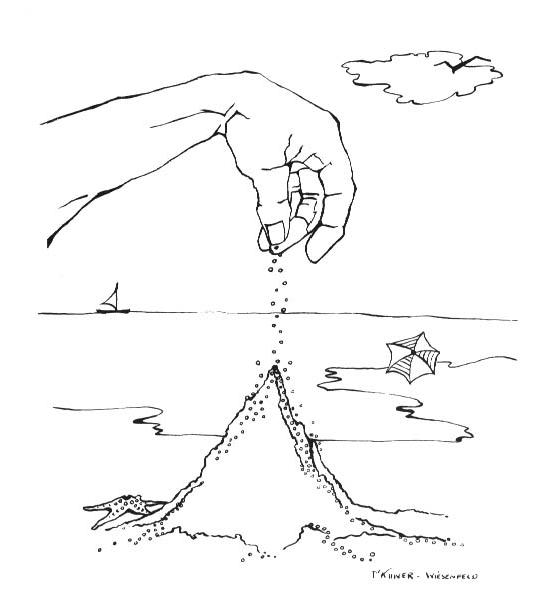
\includegraphics[scale=.25]{mano.jpg}
		}
		& \\

& \\ 		& \\ 
		& �Gracias! \\
		& \\
	\end{tabular}

\end{frame}



\end{document}


